\documentclass[../TinyBot.tex]{subfiles}
\begin{document}

\section{Construction} \label{sec:construction}

The first step is to cut out your base material. This can be any material stiff enough to support the Arduino, breadboard, and motors. The club provides corflute, though other materials such as wood or plastic from milk bottles can be used if desired. The base can be any shape, though ensure it is big enough to fit the breadboard, the Arduino you are using if not using a Nano, and a battery.
It is useful to lay out the components you are using on the base material before cutting. \\

\begin{notebox}
    Get creative with the shape of your robot base! Make it a diamond, some kind of squiggle, any shape that fits the components will do!    
\end{notebox}

Once you have cut out the base, peel the backing paper from the breadboard and stick the breadboard to the base.
\begin{center}
    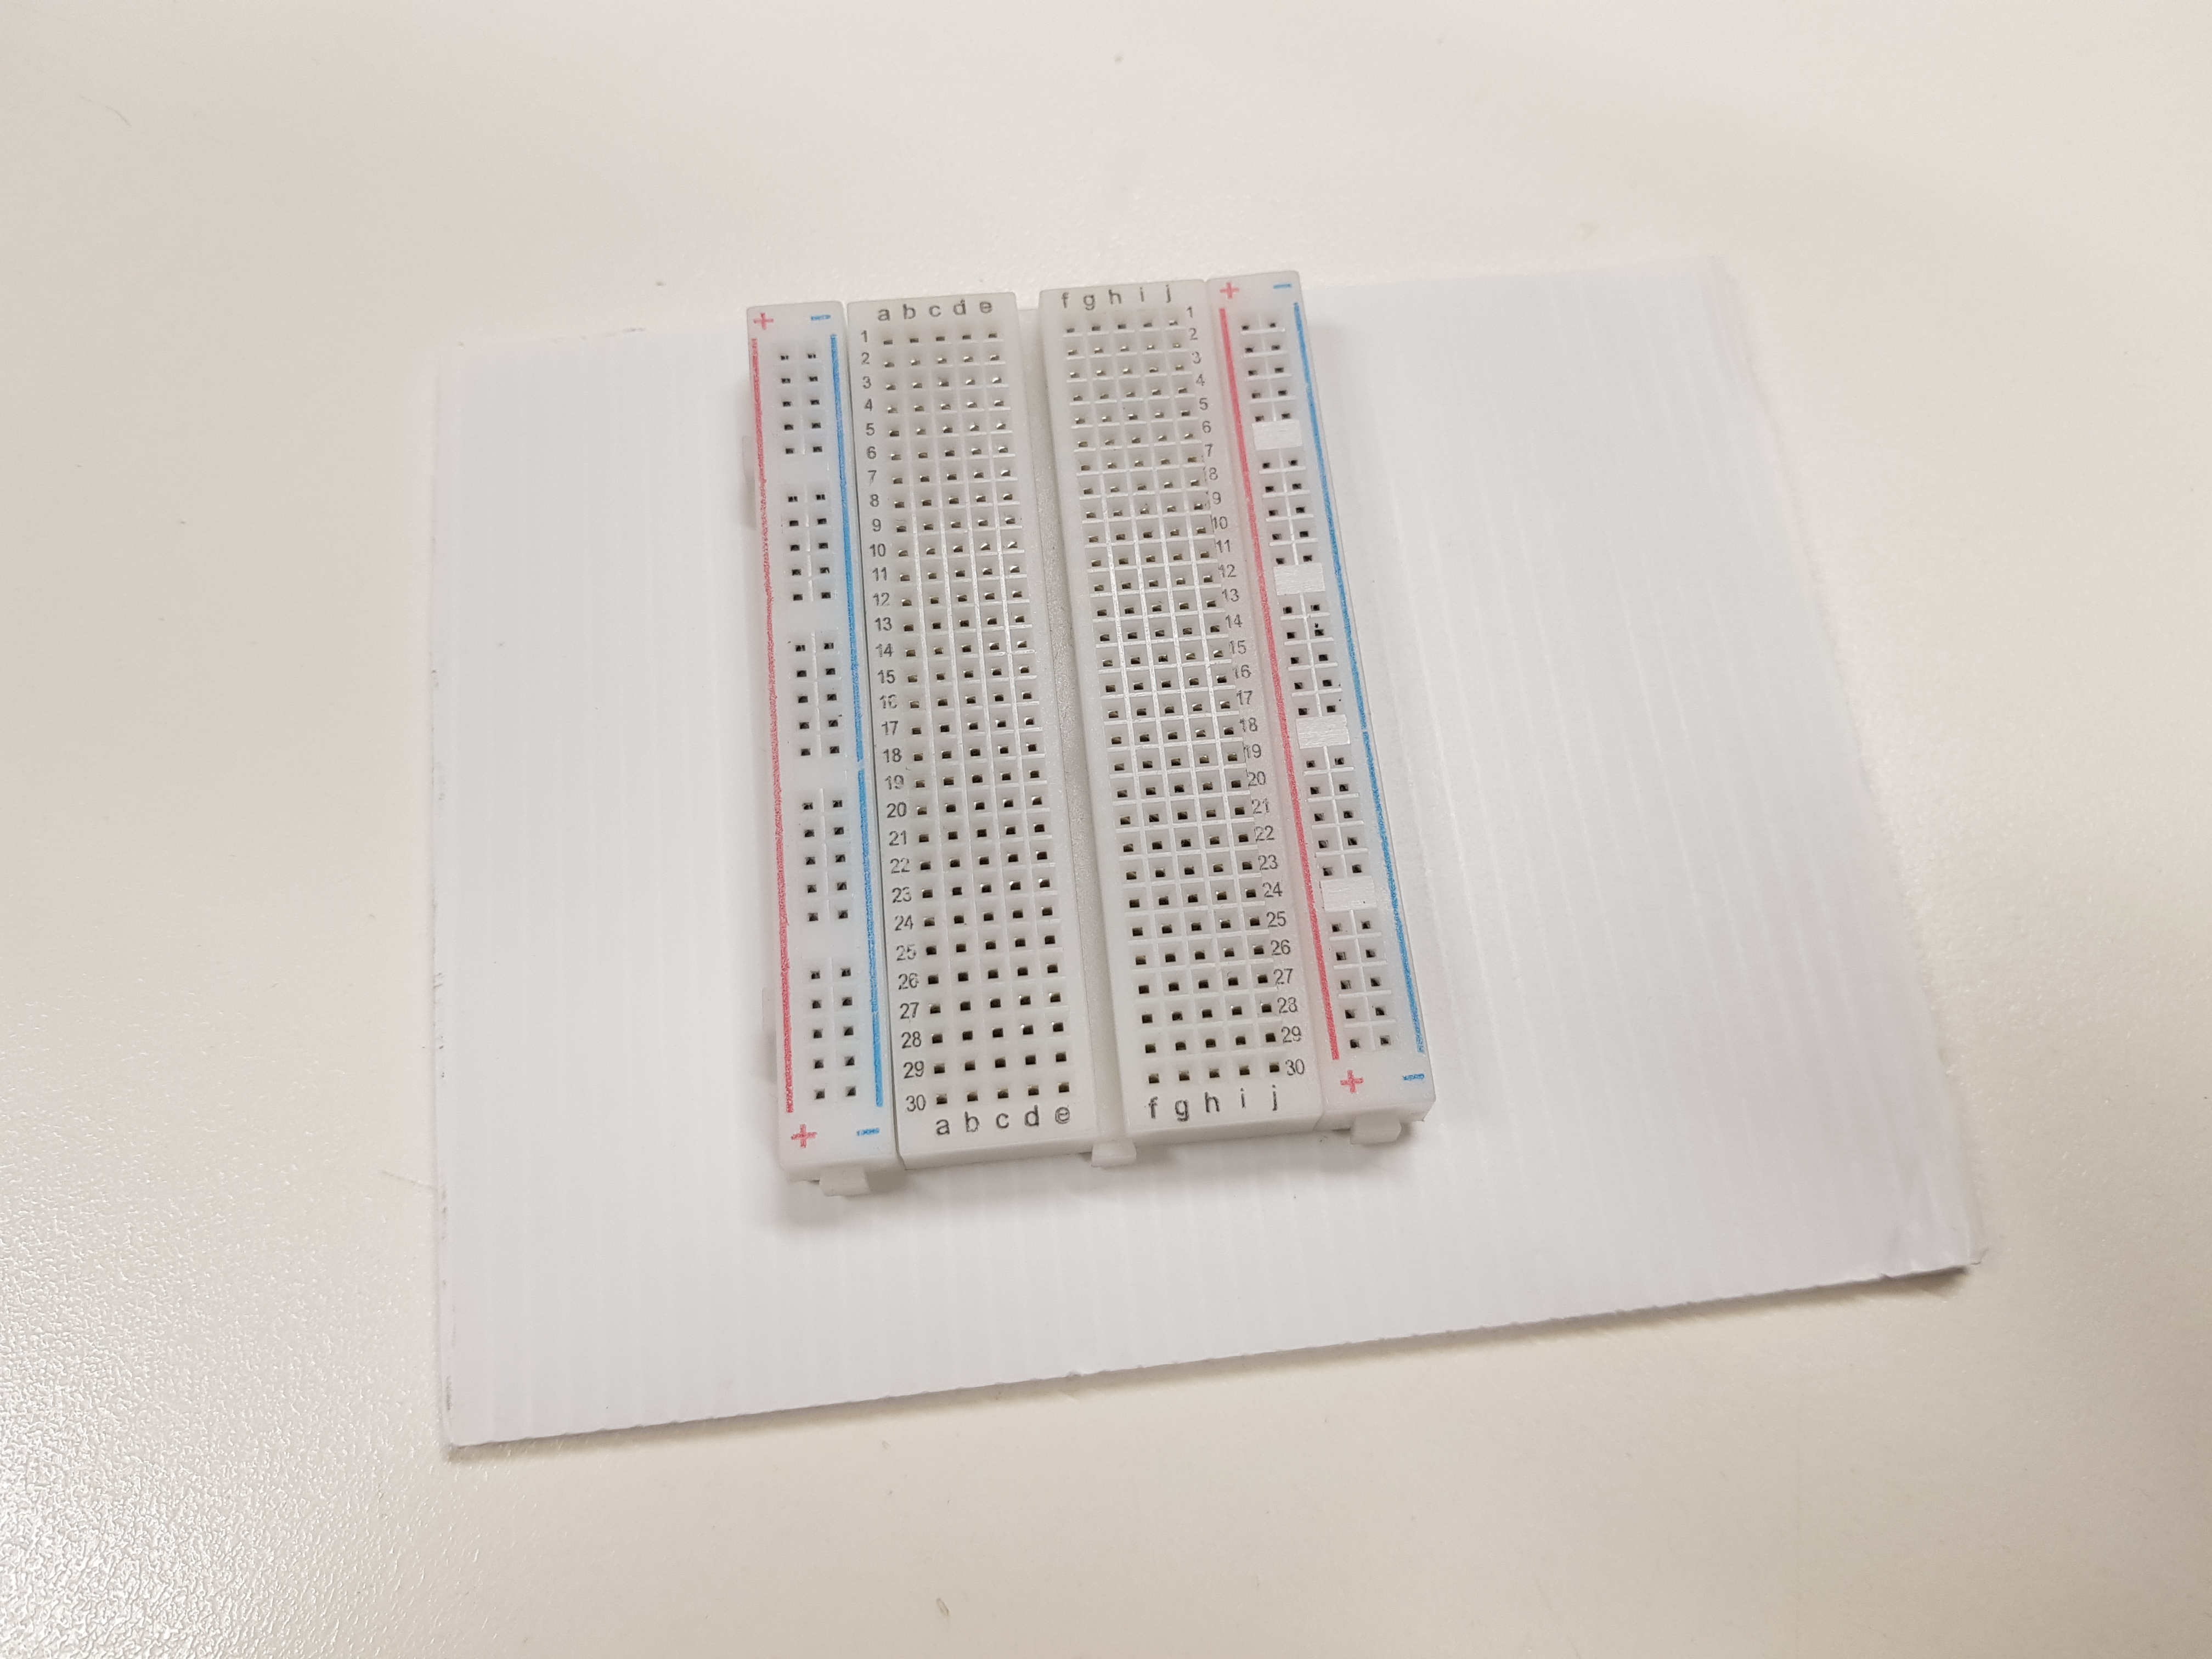
\includegraphics[width=0.6\linewidth]{breadboard_on_base.jpg}
    % \captionof{figure}{fig:construction:breadboard-on-base}
    % \label{fig:construction:breadboard-on-base}
\end{center}

Then place the motor covers and caster wheel on the base and mark out where holes need to be made. The club has plenty of motor covers, though cable ties can be used as an alternative to secure the motors. \\
If using a material like corflute the holes can be marked/made with a screwdriver. Holes will have to be marked and made differently if using other materials. 
\begin{center}
    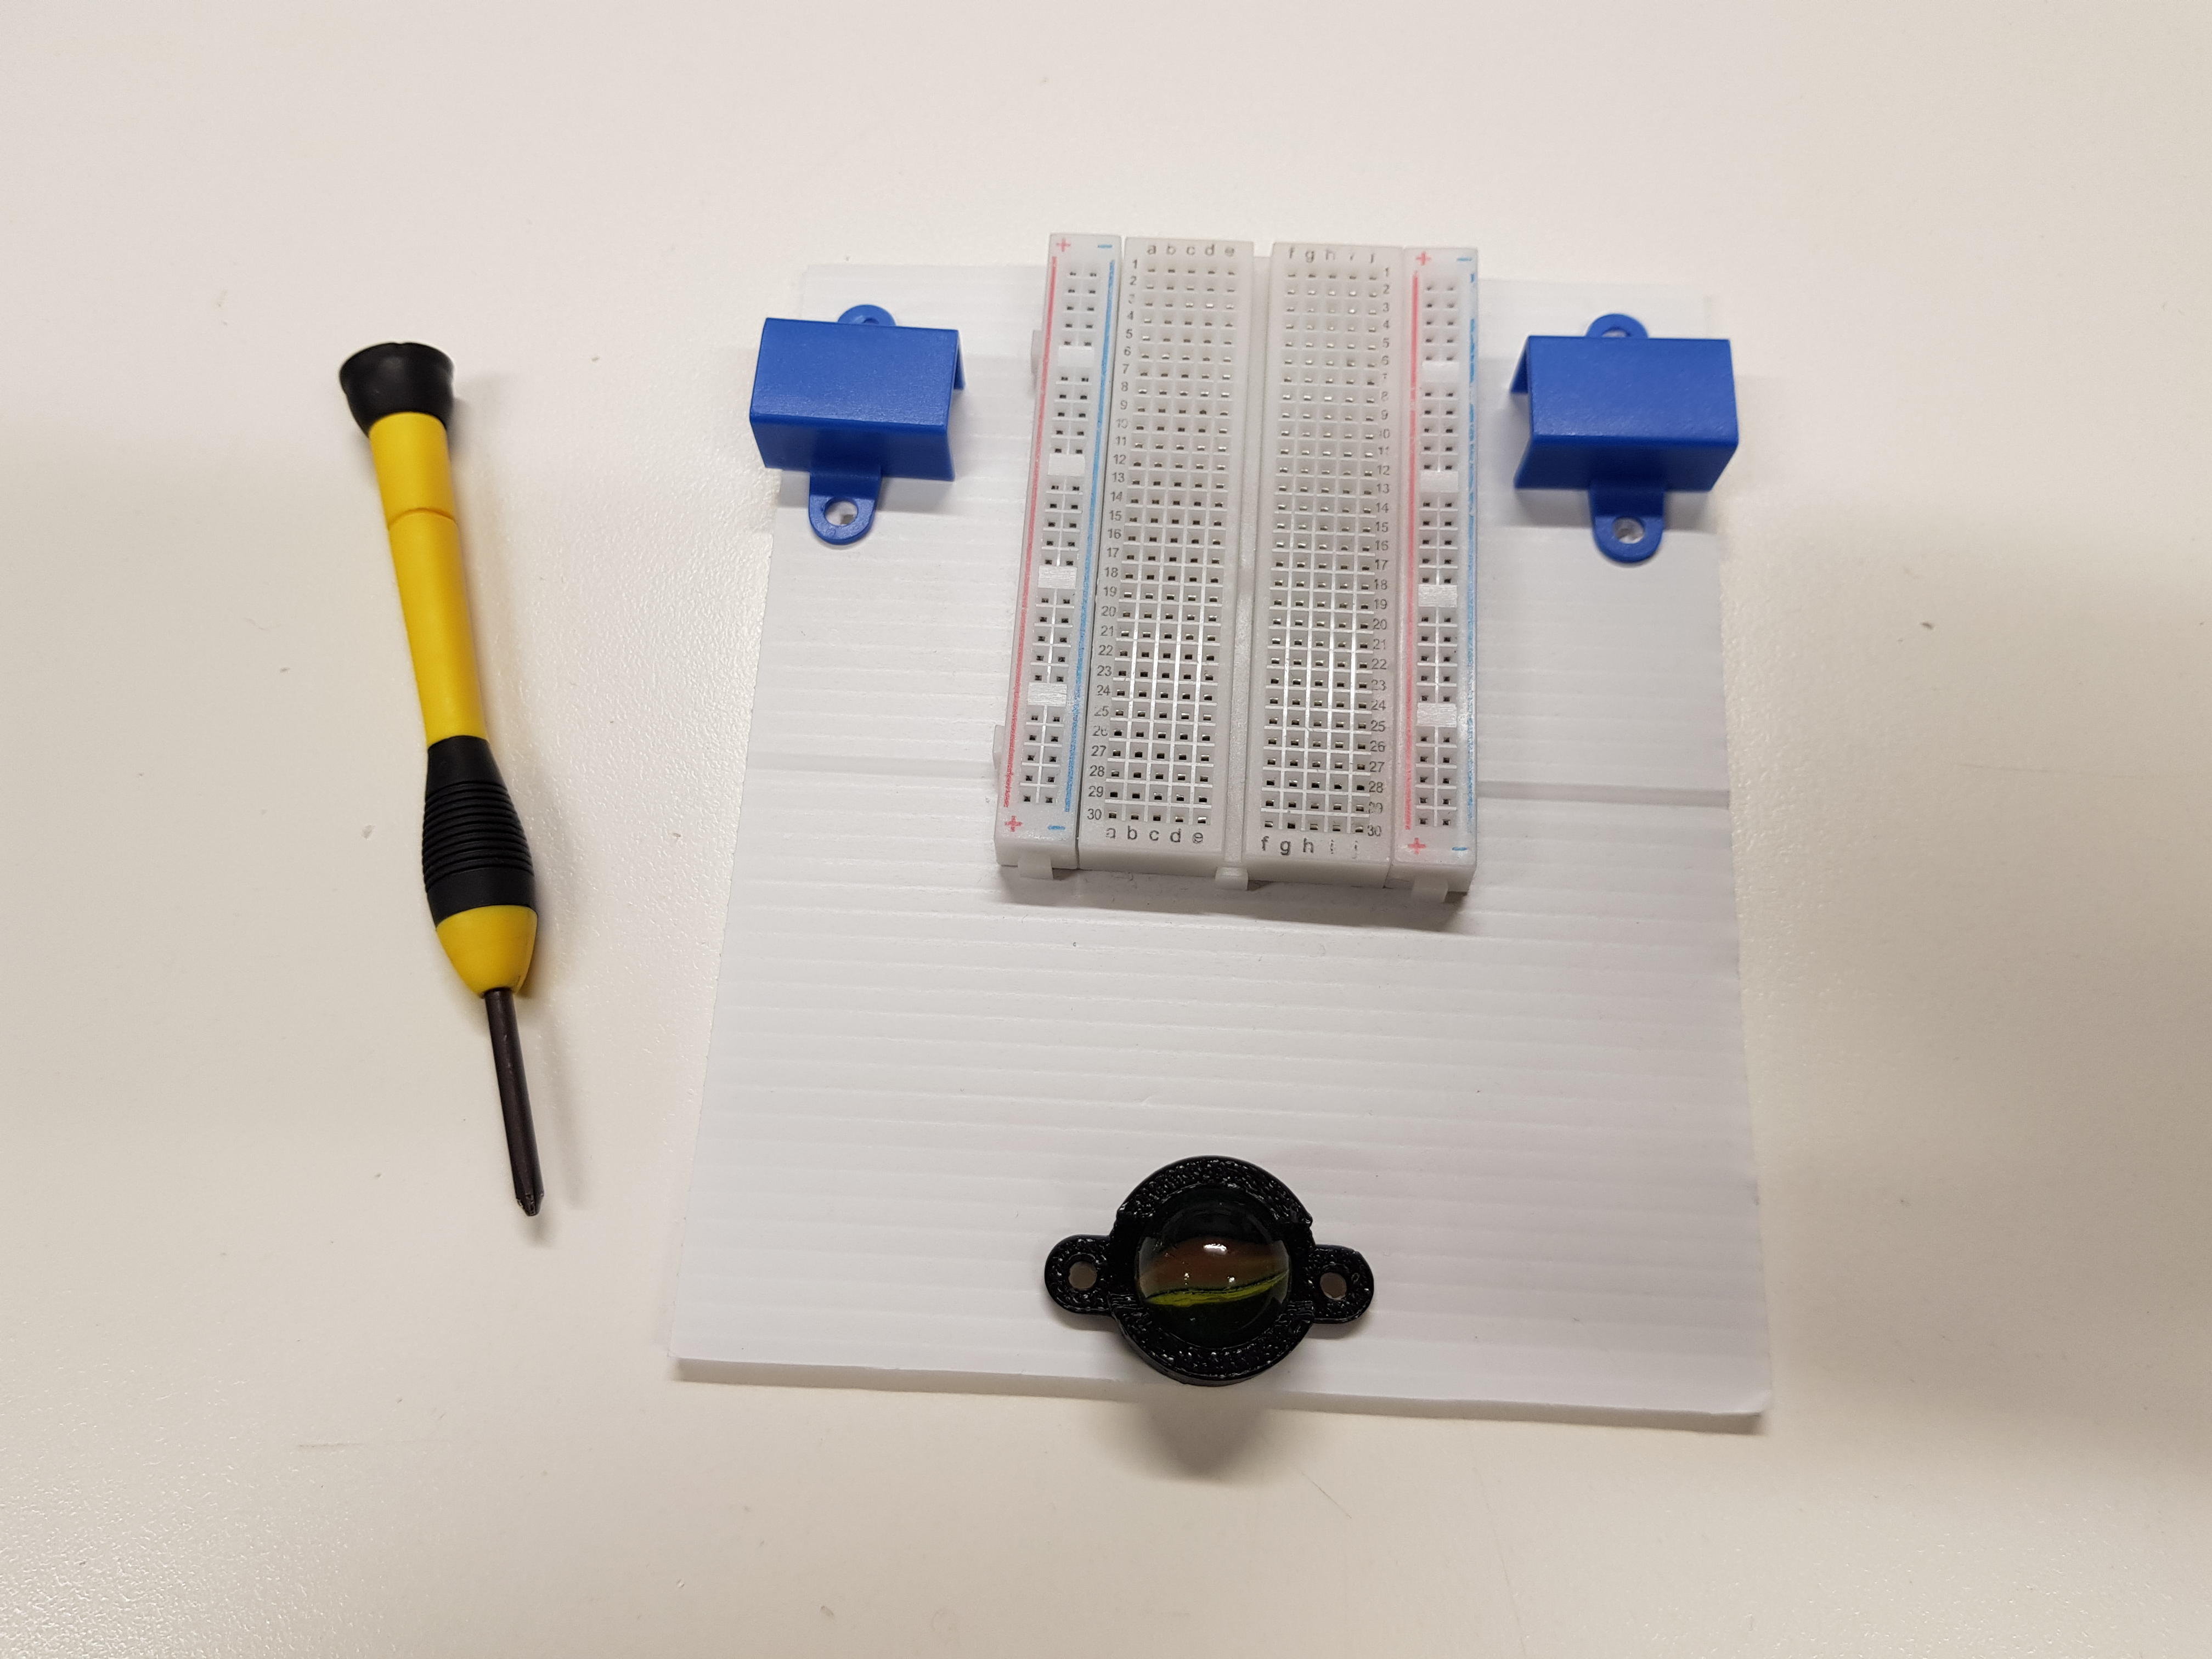
\includegraphics[width=0.6\linewidth]{lining_up_holes_base_screwdriver.jpg}
\end{center}

\begin{center}
    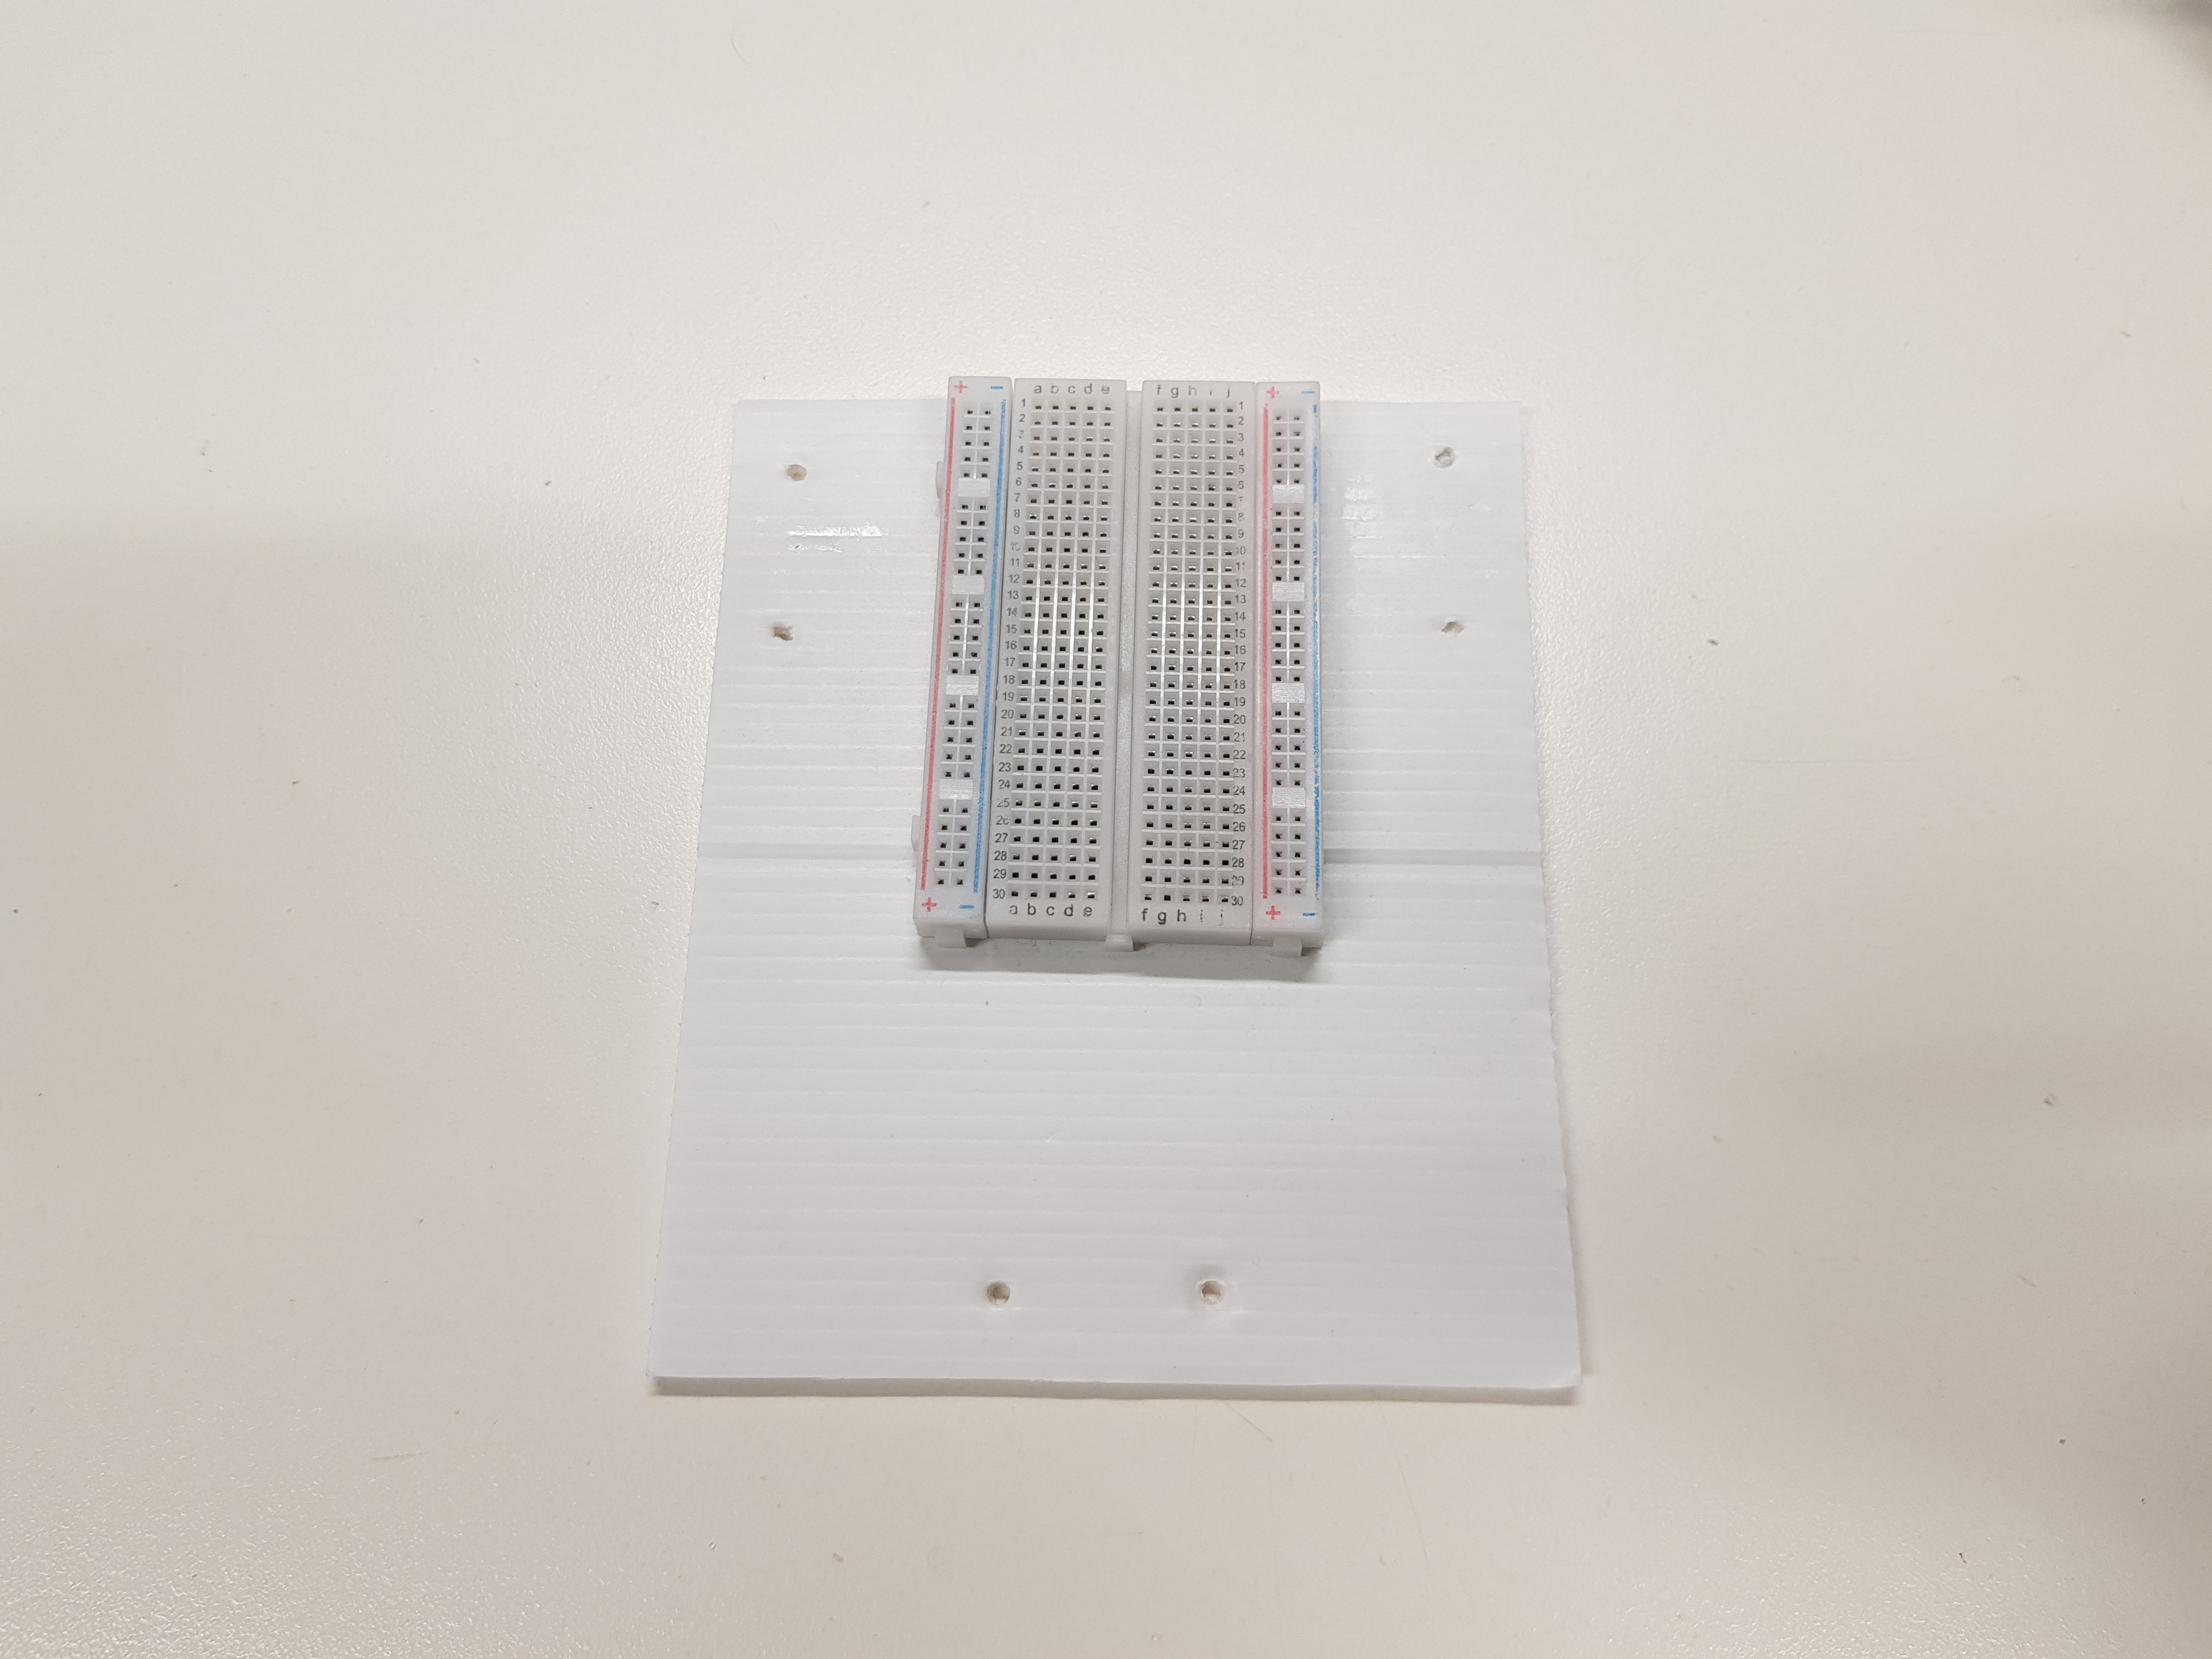
\includegraphics[width=0.6\linewidth]{base_with_holes.jpg}
\end{center}

It is easier to wire the circuit after the breadboard is stuck to the base as you don't have to worry about pulling any wires out when sticking on the breadboard. The full wiring diagram, with a battery, is shown below. Before starting to wire up the circuit, double check your H-Bridge is in fact a H-Bridge; a lot of IC chips look really similar and are difficult to tell apart. On the back of your chip there should be some serial numbers, make sure that one of these numbers is L293D - there are lots of variations of this H-Bridge so numbers like L293DE are also valid H-Bridges. \\

Make sure to check which wire is the positive wire on the motor you have, it should be written on the back plate of the motor. Plugging the motor in backwards will not break anything, the motor will just spin backwards. 

Swapping the motor direction can be done by swapping the green and yellow wires attached to the motor. 


\begin{center}
    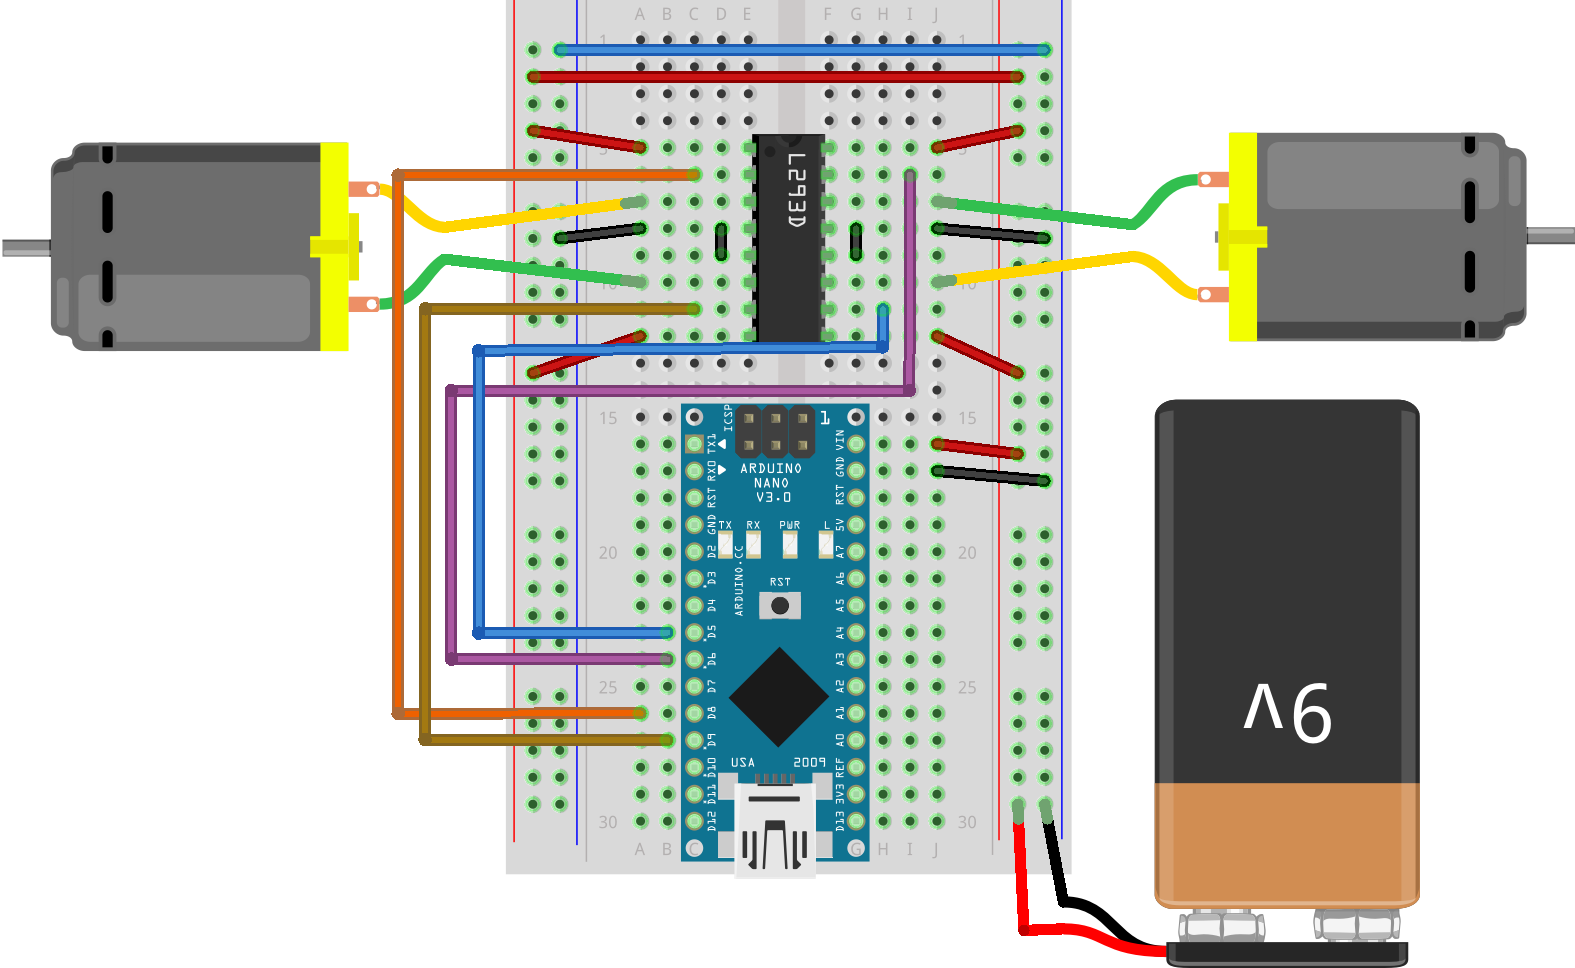
\includegraphics[width=\textwidth]{resources/H-bridge-nano_bb.png}
    \captionof{figure}{Wiring Schematic for H-Bridge}
    \label{fig:schematic-hbridge-battery}
\end{center}

If you don't have a battery, the circuit is mostly the same; though with some differences with how power is supplied to the circuit. Instead of powering the Arduino and circuit with the 9V battery you power the Arduino through USB and the circuit from the 5V output pin. See below for a wiring diagram without the battery.


\begin{center}
    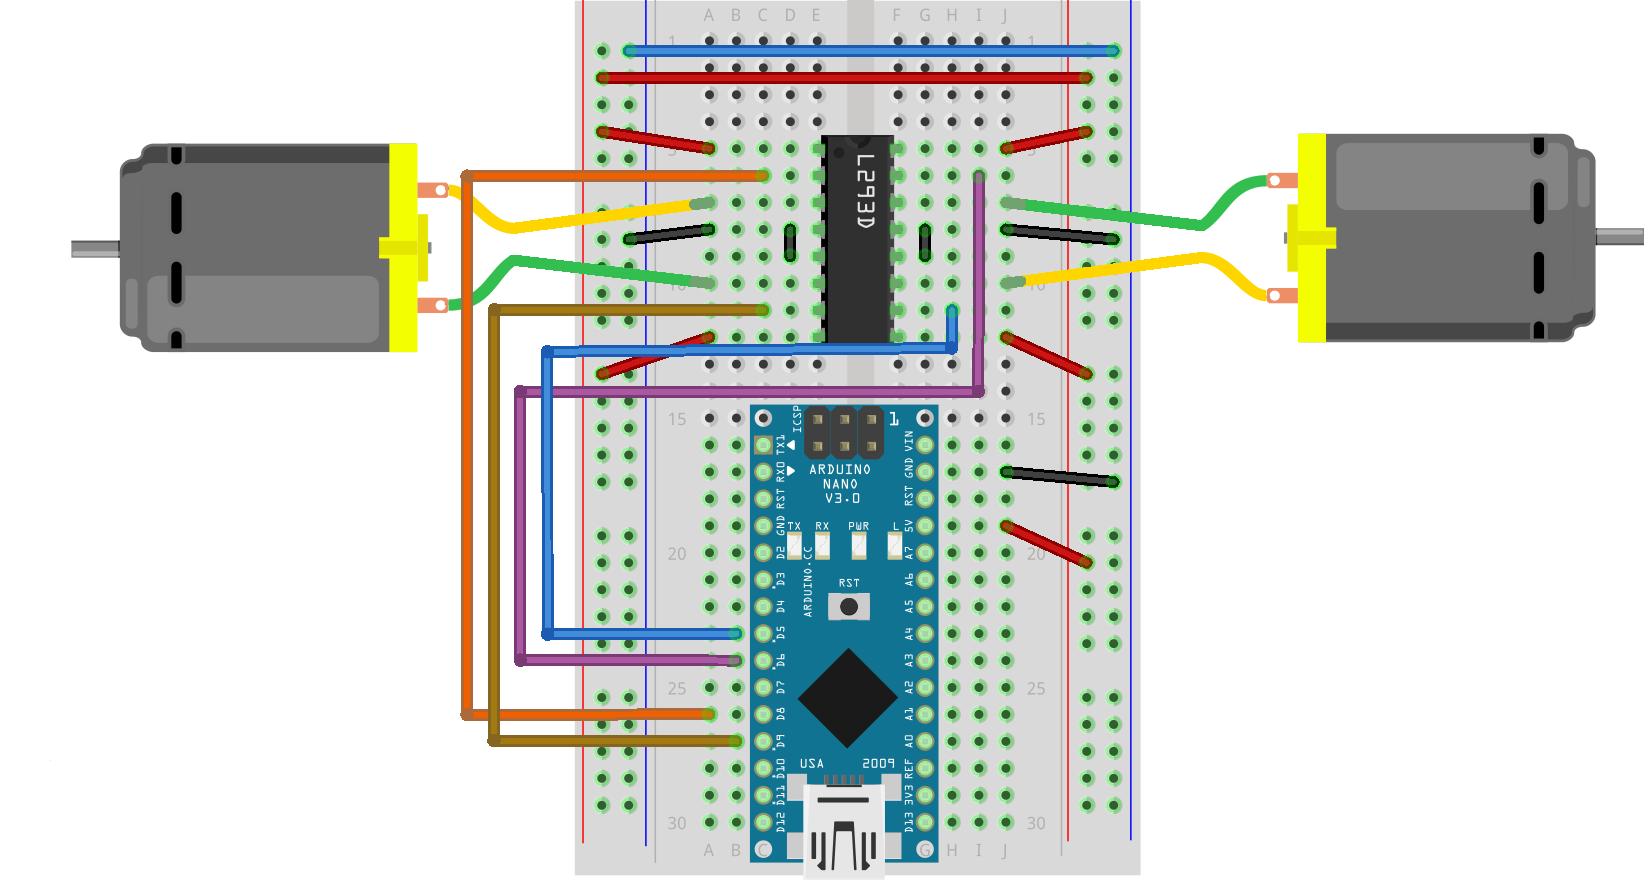
\includegraphics[width=\textwidth]{resources/H-bridge-nano-without-battery_bb.png}
    \captionof{figure}{Wiring Schematic for H-Bridge}
    \label{fig:schematic-hbridge-nobattery}
\end{center}


The circuit in real life should look something like this:

\begin{center}
    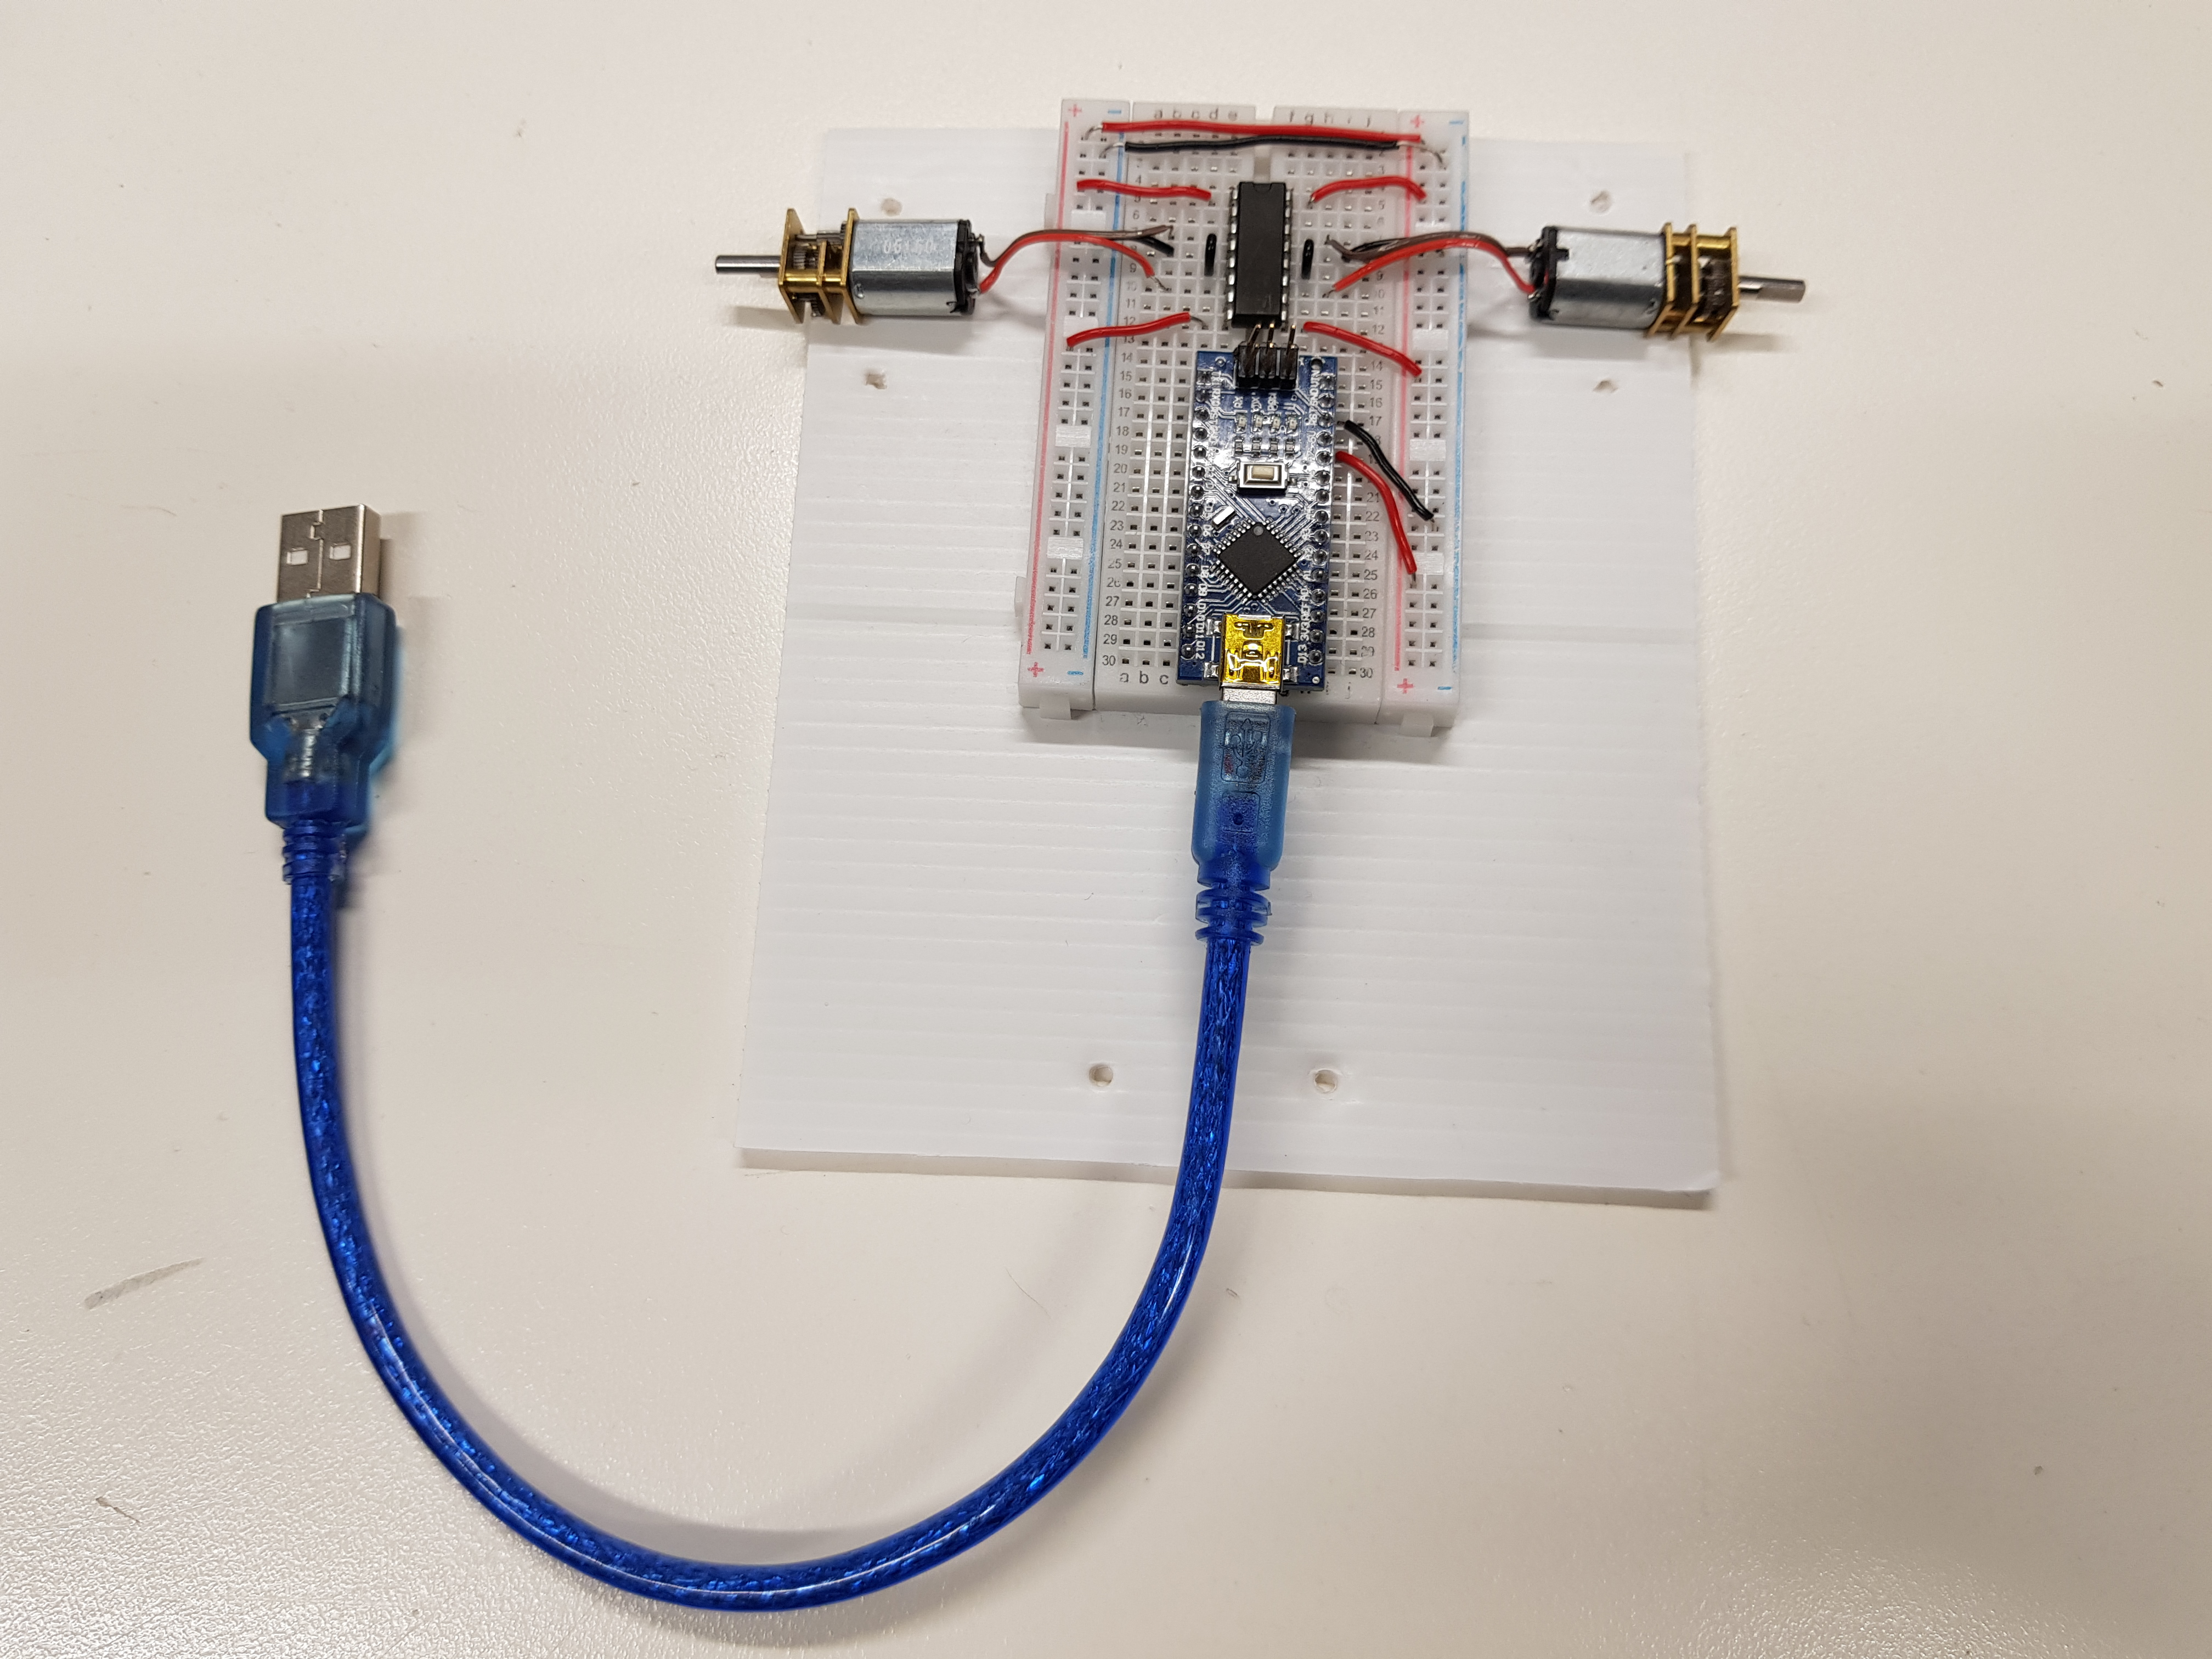
\includegraphics[width=0.6\linewidth]{circuit_on_base.jpg}
\end{center}


% \begin{center}
%     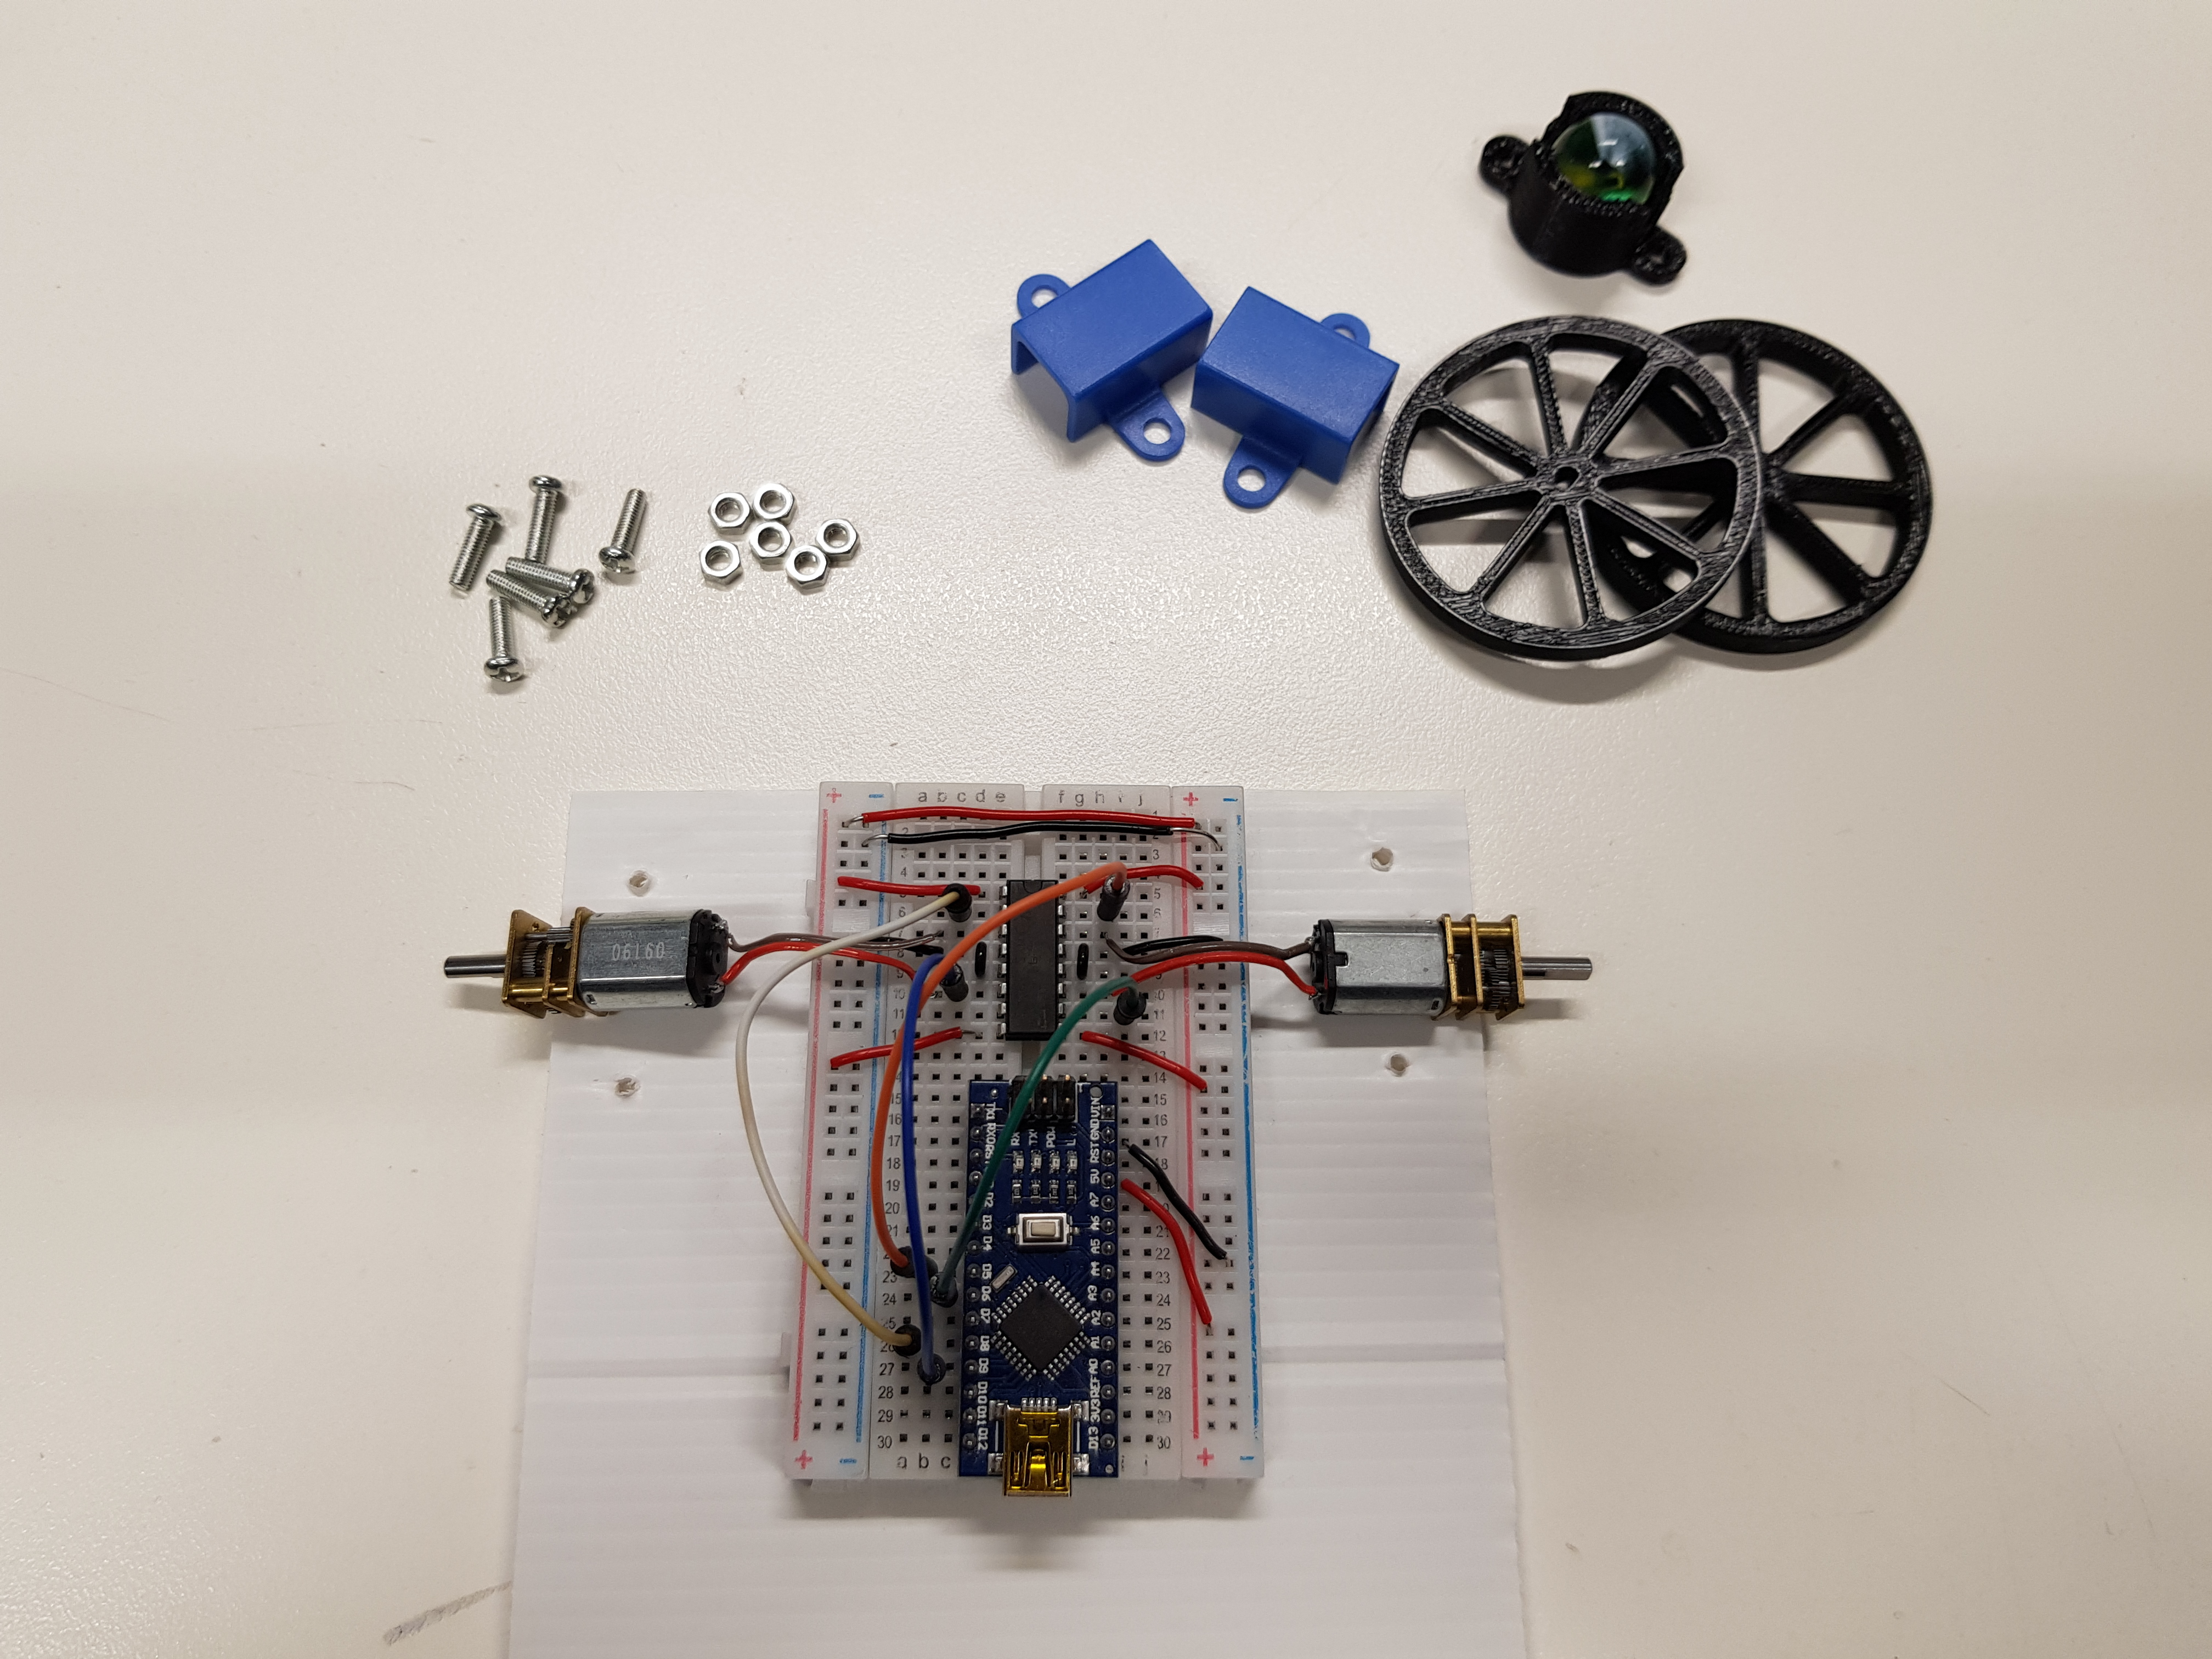
\includegraphics[width=0.6\linewidth]{wired_all_parts.jpg}
% \end{center}
Place the motor covers over the motors and attach to the base using the provided screws. The caster wheel is also attached using screws. 
% \begin{center}
%     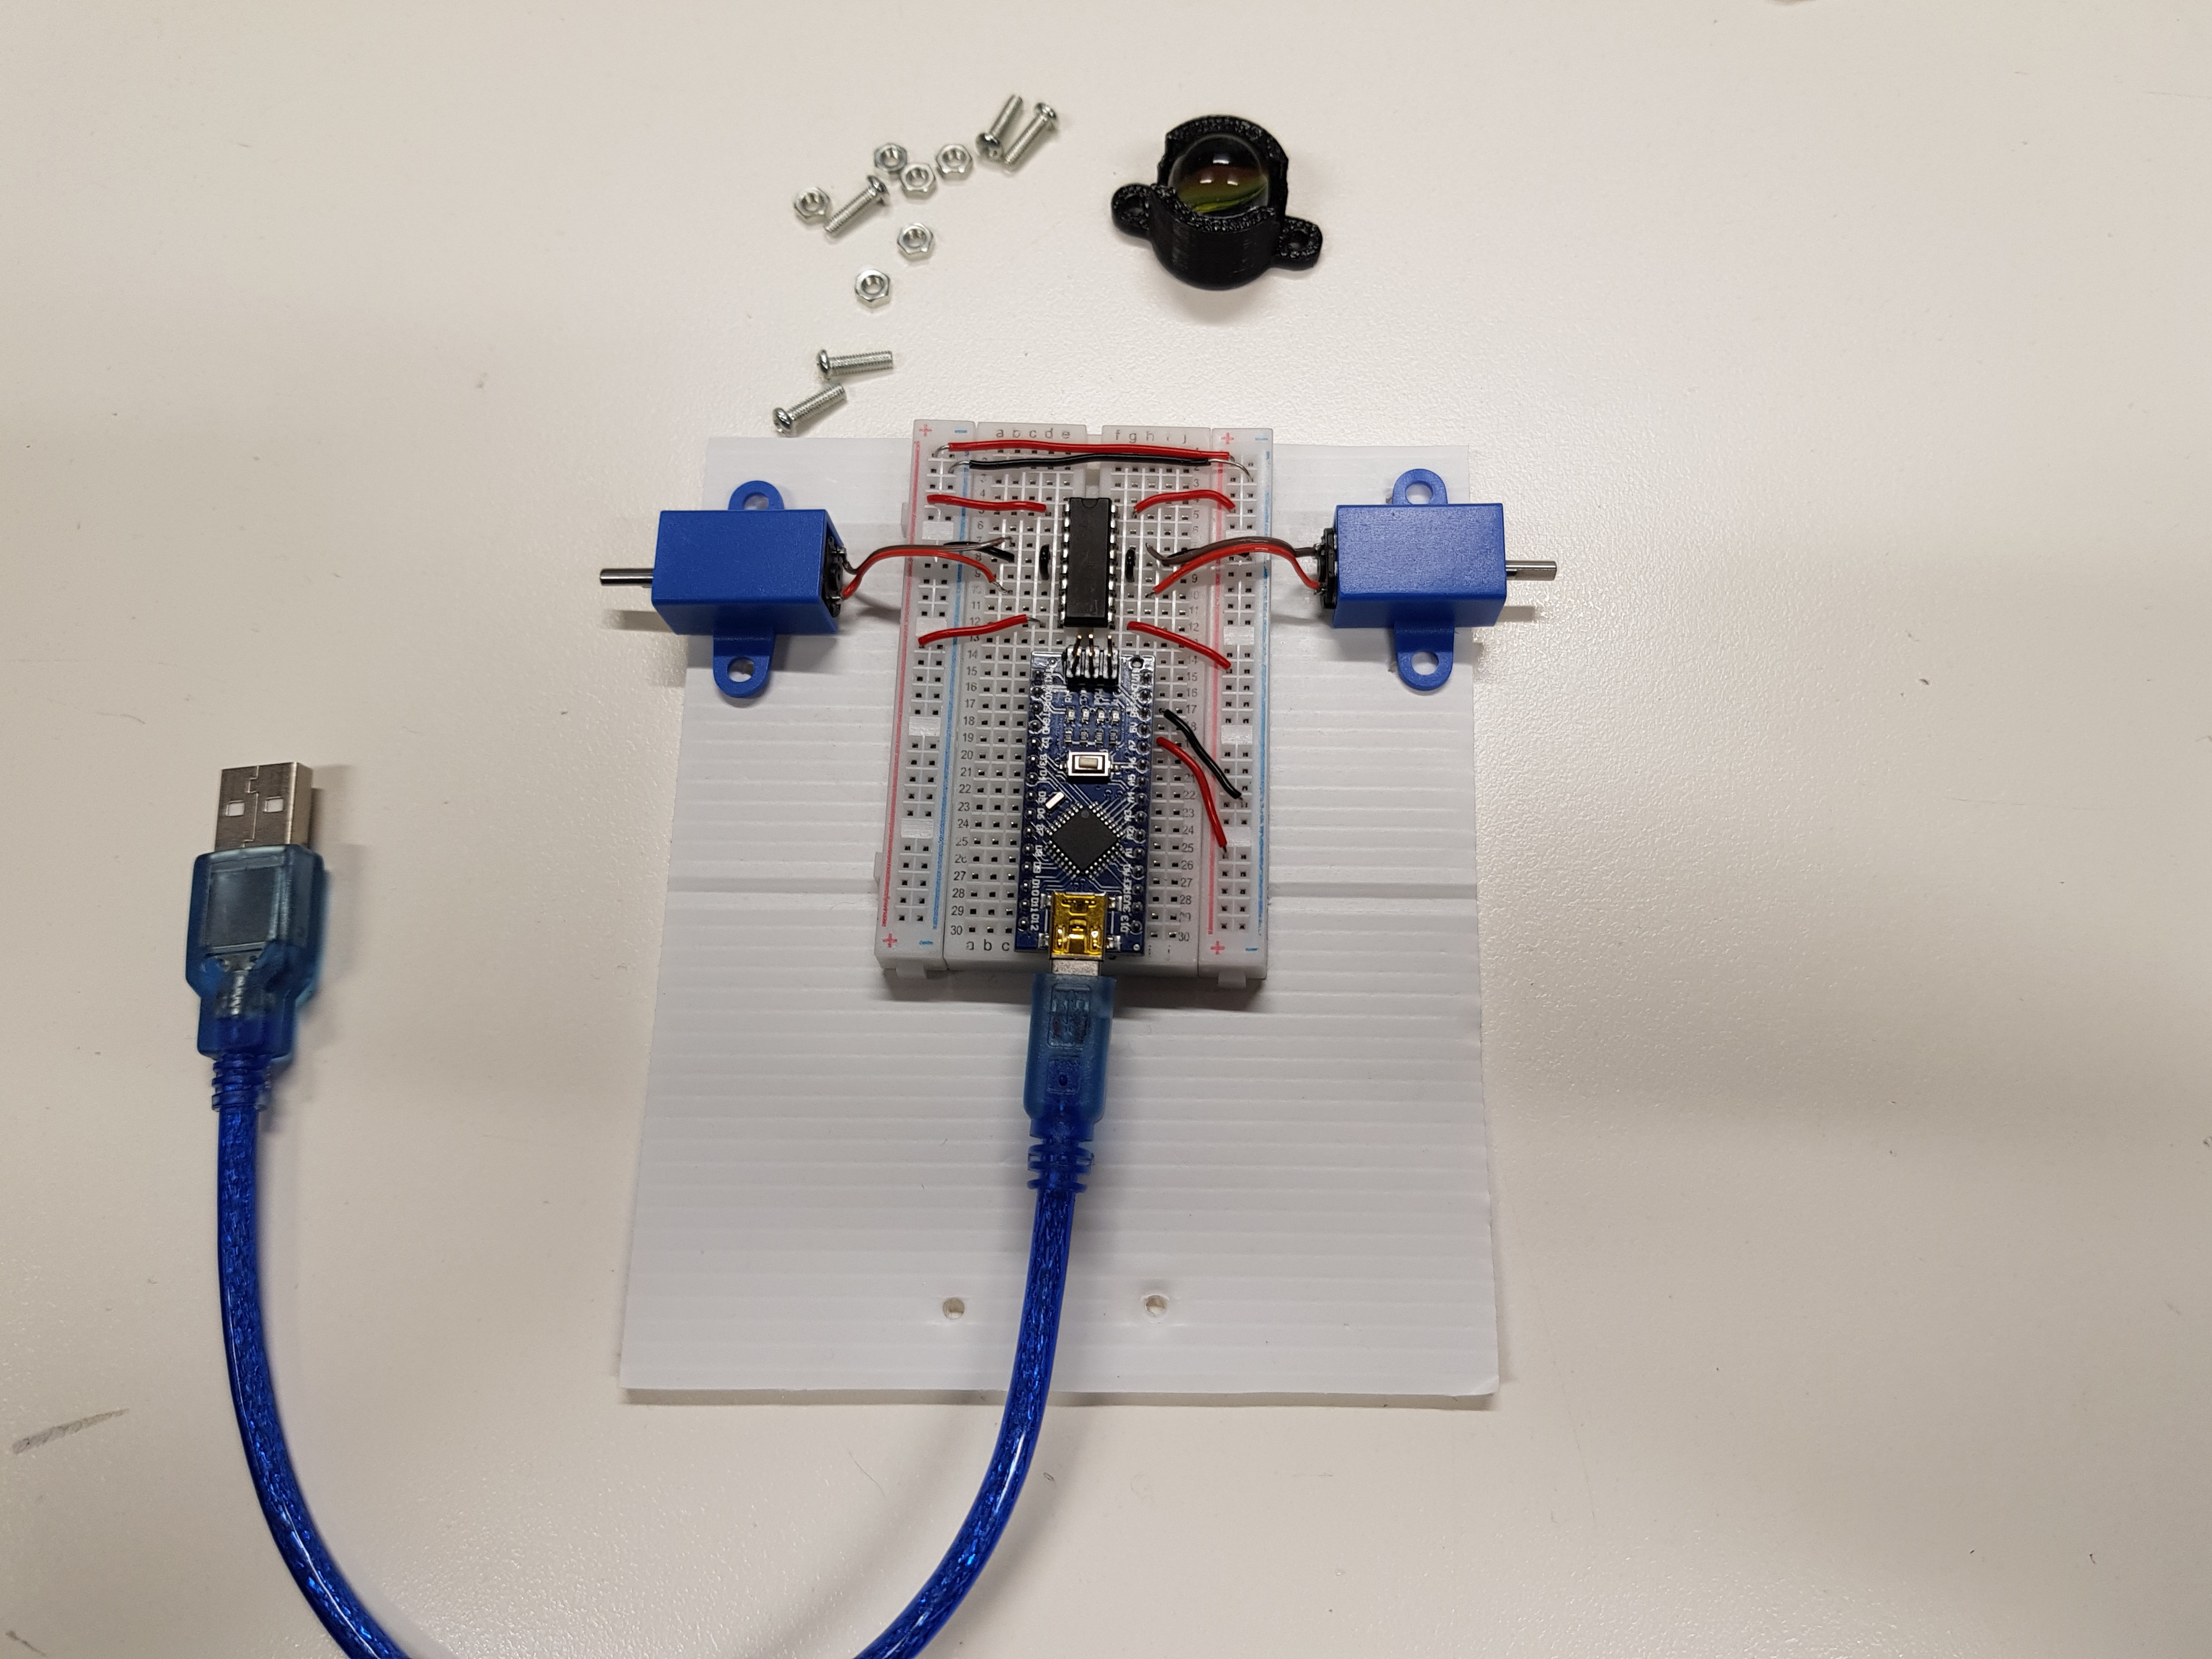
\includegraphics[width=0.6\linewidth]{circuit_base_all_parts_minus_wheels.jpg}
% \end{center}

\begin{center}
    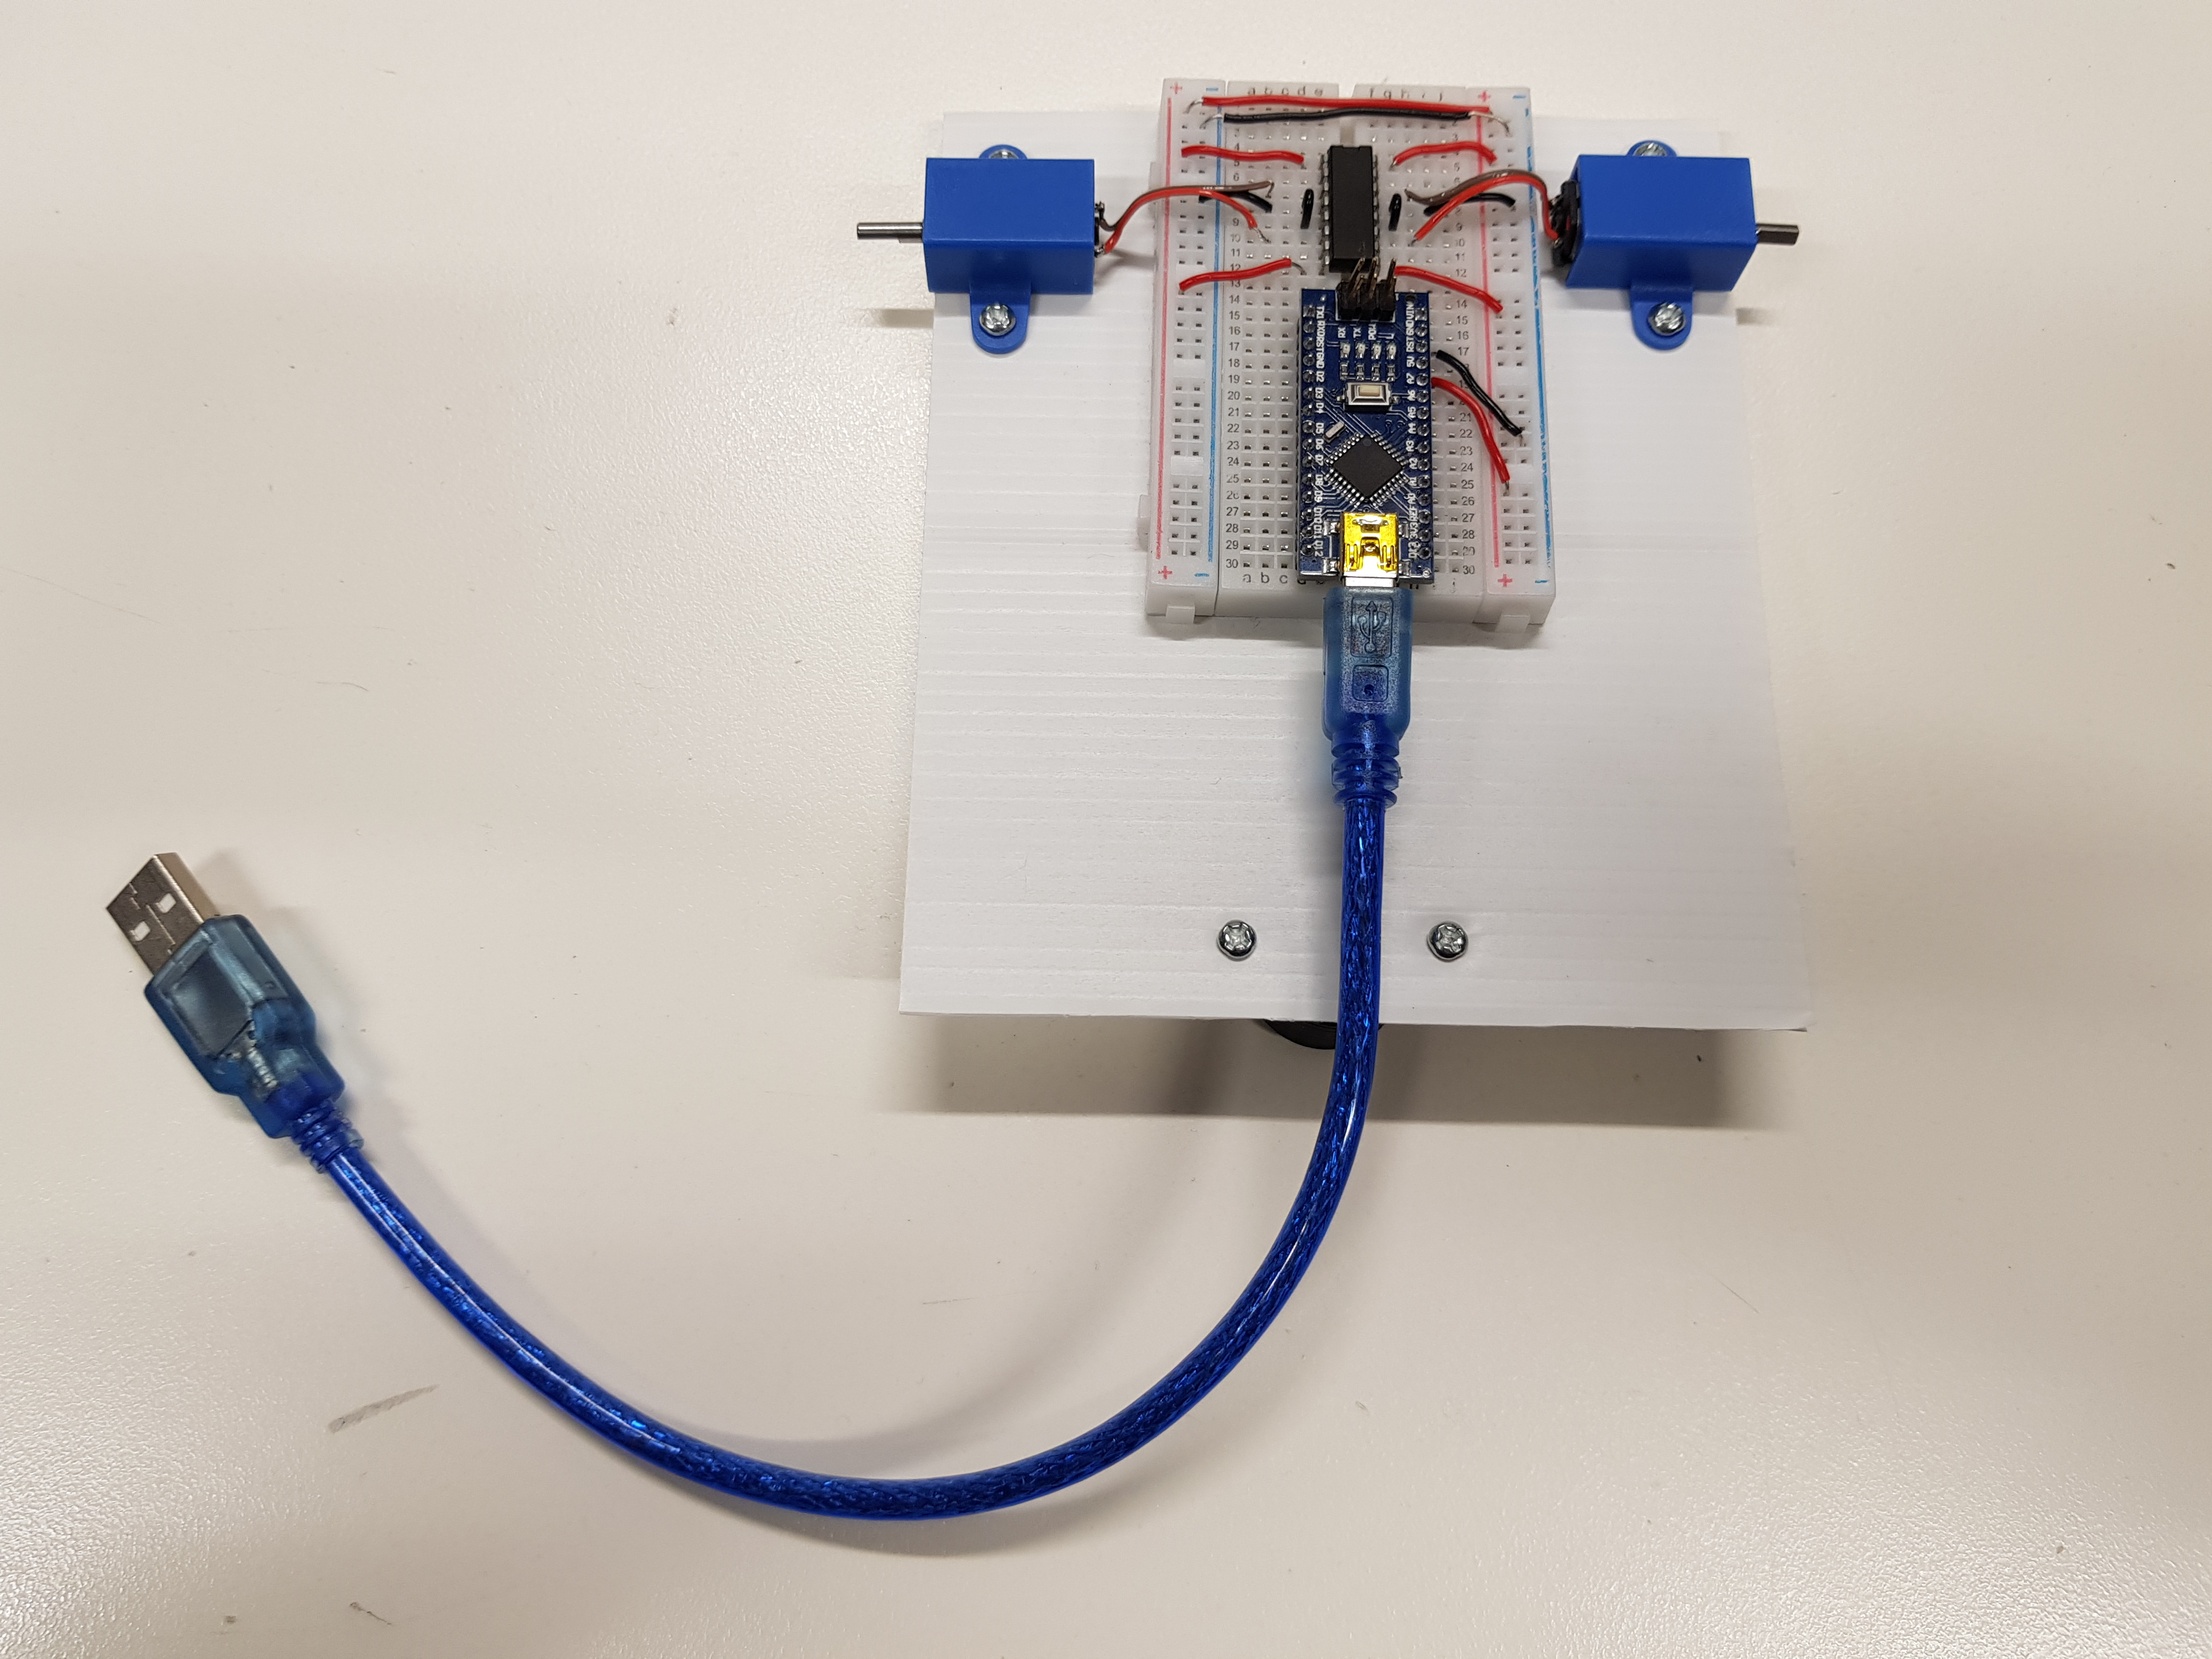
\includegraphics[width=0.6\linewidth]{cover_and_caster_screws.jpg}
\end{center}

Your TinyBot is now fully assembled.
\begin{center}
    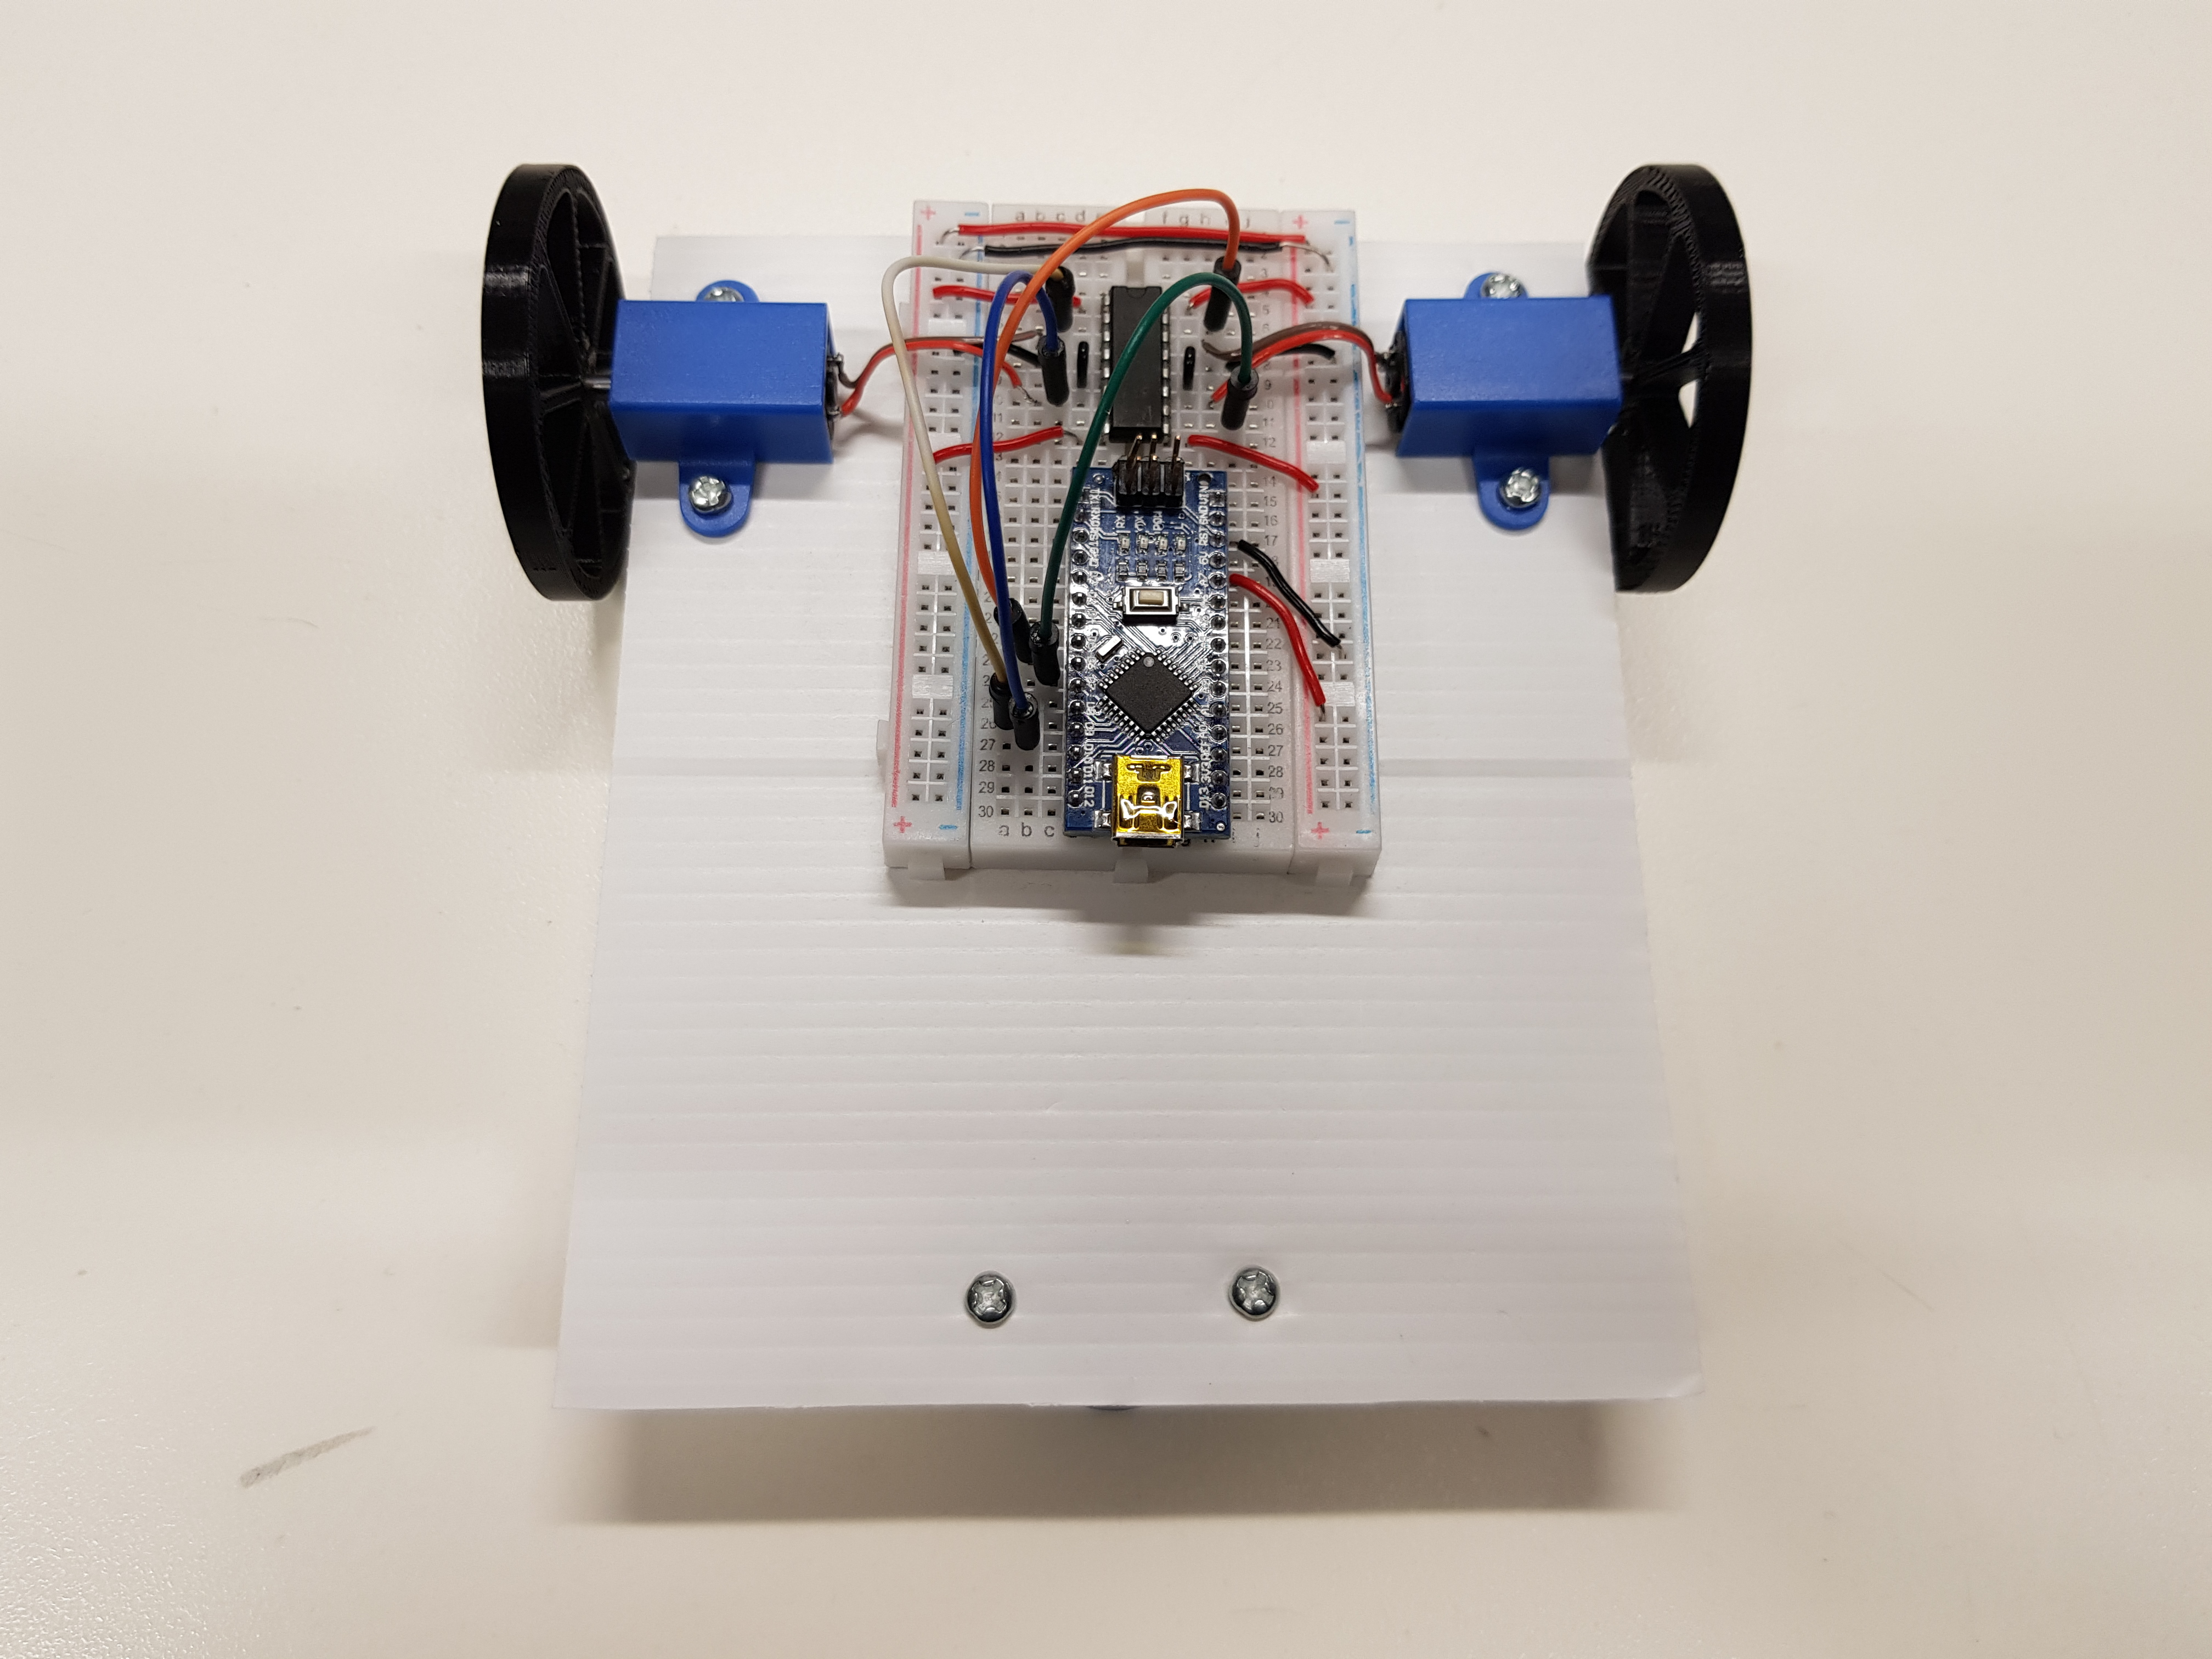
\includegraphics[width=0.6\linewidth]{final_assembled.jpg}
\end{center}

\end{document}